\documentclass[10pt]{article}
% Shared preamble for the second-brain PDF handouts.  Compile with:  latexmk -pdf -outdir=build <file>.tex
\usepackage[T1]{fontenc}
\usepackage{lmodern}
\usepackage[a4paper,margin=18mm]{geometry}
\usepackage{amsmath,amssymb,mathtools,bm}
\usepackage{siunitx}
\sisetup{per-mode=symbol,detect-all}
\usepackage{booktabs,array,enumitem}
\usepackage{xcolor}
\usepackage{tikz}
\usetikzlibrary{arrows.meta,calc,angles,quotes,decorations.pathreplacing,positioning}
\usepackage{pgfplots}
\pgfplotsset{compat=1.18}
\usepackage[most]{tcolorbox}
\usepackage[colorlinks=true,linkcolor=blue!50!black,urlcolor=blue!50!black]{hyperref}

% palette shared with the figures (dataviz reference, light mode)
\definecolor{cBlue}{HTML}{2A78D6}
\definecolor{cOrange}{HTML}{EB6834}
\definecolor{cAqua}{HTML}{1BAF7A}
\definecolor{cViolet}{HTML}{6250D6}
\definecolor{cRed}{HTML}{E34948}
\definecolor{cInk}{HTML}{0B0B0B}
\definecolor{cMuted}{HTML}{52514E}

% boxes mirroring the Obsidian callouts
\newtcolorbox{keybox}[1][]{enhanced,colback=violet!5,colframe=cViolet,fonttitle=\bfseries,title={#1},boxrule=0.6pt,arc=2pt,left=4pt,right=4pt}
\newtcolorbox{derivbox}[1][]{enhanced,colback=black!3,colframe=cMuted,fonttitle=\bfseries,title={#1},boxrule=0.6pt,arc=2pt,left=4pt,right=4pt}
\newtcolorbox{extrabox}[1][]{enhanced,colback=blue!4,colframe=cBlue,fonttitle=\bfseries,title={Extra (beyond): #1},boxrule=0.6pt,arc=2pt,left=4pt,right=4pt}
\newtcolorbox{verifybox}[1][]{enhanced,colback=yellow!10,colframe=orange!70!black,fonttitle=\bfseries,title={Check: #1},boxrule=0.6pt,arc=2pt,left=4pt,right=4pt}

\newcommand{\dd}{\mathrm{d}}
\newcommand{\DD}{\mathrm{D}}
\newcommand{\vect}[1]{\bm{#1}}
\setlength{\parindent}{0pt}
\setlength{\parskip}{4pt}

\title{Climate, Part I: energy balance and feedback\\\large formula sheet, derivations and worked numbers}
\author{second brain $\cdot$ chapters CL03 and CL04}
\date{}
\begin{document}
\maketitle
\vspace{-2em}

\section*{1. Radiation laws}
\begin{tabular}{@{}lll@{}}
\toprule
Planck & $B_\lambda=\dfrac{2hc^2}{\lambda^5}\,\dfrac{1}{e^{hc/\lambda k_BT}-1}$ & limits: Wien tail, Rayleigh--Jeans $2ck_BT/\lambda^4$\\[6pt]
Wien & $\lambda_mT=\SI{2898}{\micro\metre\kelvin}$ & Sun \SI{0.50}{\micro\metre}; \SI{255}{K}: \SI{11.4}{\micro\metre}\\[2pt]
Stefan--Boltzmann & $F=\sigma T^4$, $\sigma=\dfrac{2\pi^5k_B^4}{15h^3c^2}=\SI{5.670e-8}{\watt\per\square\metre\per\kelvin\tothe{4}}$ & \SI{316}{\watt\per\square\metre} at \SI{273}{K}\\
Solar irradiance & $S=\sigma T_\odot^4(R_\odot/d)^2=\SI{1361}{\watt\per\square\metre}$ & $S/4=\SI{340}{\watt\per\square\metre}$\\
\bottomrule
\end{tabular}

\begin{keybox}[Zero-dimensional balance]
\[
\frac{S(1-\alpha)}{4}=\sigma T_e^4\qquad\Longrightarrow\qquad T_e=\Bigl[\frac{S(1-\alpha)}{4\sigma}\Bigr]^{1/4}=\SI{254.6}{K}\quad(\alpha=0.30).
\]
\end{keybox}

\begin{center}
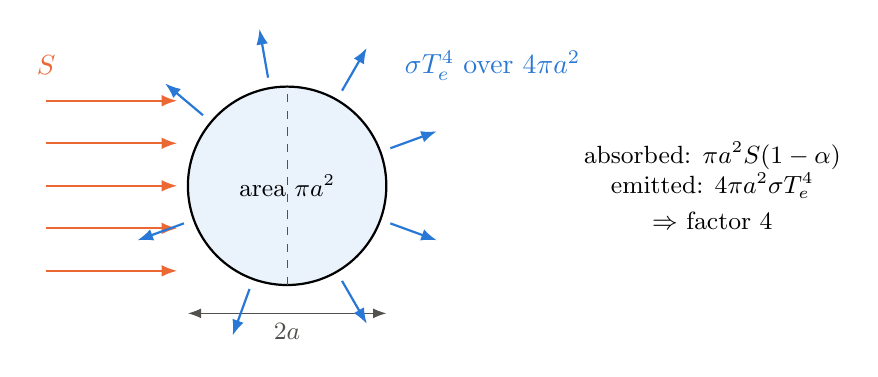
\begin{tikzpicture}[scale=0.9]
  % incoming parallel beam on a disc of radius a, emission from the whole sphere
  \def\a{1.4}
  \foreach \y in {-1.2,-0.6,0,0.6,1.2}{\draw[-{Latex[length=2mm]},cOrange,thick] (-3.4,\y) -- (-1.55,\y);}
  \draw[thick,fill=cBlue!10] (0,0) circle (\a);
  \draw[dashed,cMuted] (0,-\a) -- (0,\a);
  \node[cOrange] at (-3.4,1.7) {$S$};
  \node at (0,0) {\small area $\pi a^2$};
  \draw[{Latex}-{Latex},cMuted] (-\a,-1.8) -- (\a,-1.8) node[midway,below] {\small $2a$};
  \foreach \t in {20,60,100,140,200,250,300,340}{\draw[-{Latex[length=2mm]},cBlue,thick] ({1.55*cos(\t)},{1.55*sin(\t)}) -- ({2.25*cos(\t)},{2.25*sin(\t)});}
  \node[cBlue] at (2.9,1.7) {$\sigma T_e^4$ over $4\pi a^2$};
  \node[align=center,font=\small] at (6.0,0) {absorbed: $\pi a^2S(1-\alpha)$\\emitted: $4\pi a^2\sigma T_e^4$\\[2pt]$\Rightarrow$ factor $4$};
\end{tikzpicture}
\end{center}

\begin{tabular}{@{}lrrrrr@{}}
\toprule
 & $S$ (\si{\watt\per\square\metre}) & $\alpha$ & $T_e$ (K) & measured (K) & gap (K)\\
\midrule
Venus & 2601 & 0.77 & 227 & 737 & $+510$\\
Earth & 1361 & 0.294 & 255 & 288 & $+33$\\
Mars & 586 & 0.250 & 210 & 214 & $+4$\\
Jupiter (1 bar) & 50.3 & 0.343 & 110 & 165 & internal heat\\
\bottomrule
\end{tabular}

\smallskip
NASA Planetary Fact Sheet; $T_e$ recomputed. $\langle T^4\rangle\ge\langle T\rangle^4$ (Jensen): non-uniform planets radiate \emph{more} than the uniform estimate.

\begin{derivbox}[Relaxation time and the diurnal cycle]
$C\,\dot T=\tfrac14S(1-\alpha)-\sigma T^4$. Linearising about $T_e$: $\dot\theta=-\theta/\tau$, $\tau=C/4\sigma T_e^3$ ($4\sigma T_e^3=\SI{3.76}{\watt\per\square\metre\per\kelvin}$).
Slab \SI{7.5e5}{\joule\per\square\metre\per\kelvin}: \SI{2.3}{days}; ocean mixed layer \SI{50}{m}: \SI{1.7}{yr}.
Equatorial day cycle: mean absorbed $(1-\alpha)S/\pi=\SI{299}{\watt\per\square\metre}\Rightarrow \langle T^4\rangle^{1/4}=\SI{269.5}{K}$; first-harmonic amplitude $\tfrac12(1-\alpha)S/(C\omega)\approx\SI{8.6}{K}$.
\end{derivbox}

\section*{2. Sensitivity and feedback}
\begin{keybox}[Logarithmic differentiation and Planck sensitivity]
\[
4\frac{\Delta T}{T}=\frac{\Delta S}{S}-\frac{\Delta\alpha}{1-\alpha}\ ,\qquad
\Lambda_P=\frac{\partial T}{\partial F}=\frac{1}{4\sigma T^3}=\SI{0.27}{\kelvin\per(\watt\per\square\metre)}\ \ (\SI{3.76}{\watt\per\square\metre} \text{ per K}).
\]
\end{keybox}

Chain rule with $y_i(T)$ and $f_i\equiv\dfrac{\partial T}{\partial y_i}\dfrac{\dd y_i}{\dd T}$:
\[
\Lambda=\frac{\dd T}{\dd F}=\Lambda_P+\sum_if_i\Lambda\ \Longrightarrow\ \boxed{\Lambda=\frac{\Lambda_P}{1-\sum_if_i}}\ ,\qquad
f_\alpha=\frac{aS}{16\sigma T^3},\ \ a=-\frac{\dd\alpha}{\dd T}.
\]

\begin{verifybox}[0.27 or 0.28?]
Slide 43 writes $\Lambda_P=0.28$ together with ``3.8 W m$^{-2}$ per K''; $1/(4\sigma 255^3)=0.266$ (Wallace \& Hobbs Ex.\ 10.3 agrees). Use 0.27.
\end{verifybox}

\section*{3. Multiple steady states and hysteresis}
\[
\alpha(T)=\begin{cases}0.7&T<253\\ 0.7-\dfrac{0.5(T-253)}{40}&253\le T\le293\\ 0.2&T>293\end{cases}\qquad
\frac{S}{4}\bigl[1-\alpha(T)\bigr]=\varepsilon\sigma T^4,\ \ \varepsilon=0.6.
\]
(The slide's printed equation omits $\varepsilon=0.6$ but its code uses it; with $\varepsilon=1$ only the snowball state exists.)

\begin{center}
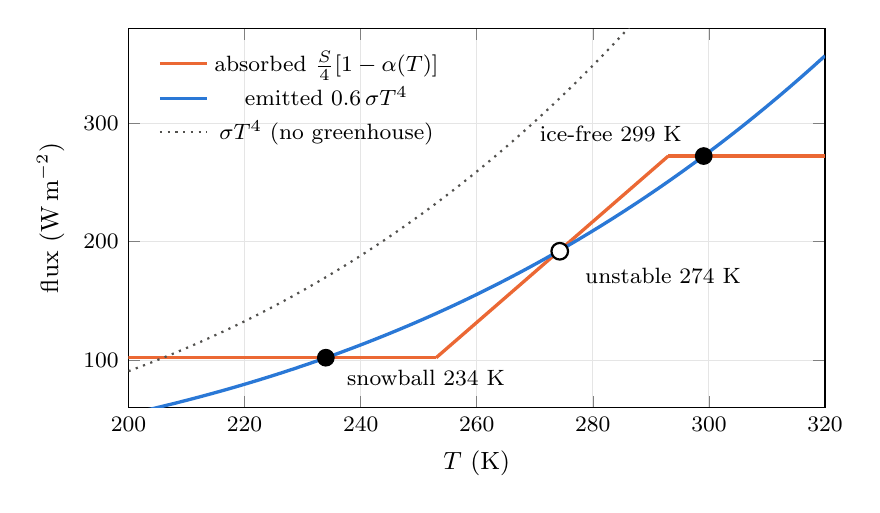
\begin{tikzpicture}
\begin{axis}[width=0.86\textwidth,height=6.4cm,xlabel={$T$ (K)},ylabel={flux (\si{\watt\per\square\metre})},xmin=200,xmax=320,ymin=60,ymax=380,
  legend style={at={(0.03,0.97)},anchor=north west,draw=none,fill=none,font=\footnotesize},grid=both,grid style={gray!20},tick label style={font=\footnotesize},label style={font=\small}]
\addplot[cOrange,very thick,domain=200:253,samples=2] {340.25*0.3};
\addplot[cOrange,very thick,domain=253:293,samples=30,forget plot] {340.25*(1-(0.7-0.5*(x-253)/40))};
\addplot[cOrange,very thick,domain=293:320,samples=2,forget plot] {340.25*0.8};
\addlegendentry{absorbed $\tfrac S4[1-\alpha(T)]$}
\addplot[cBlue,very thick,domain=200:320,samples=60] {0.6*5.670374e-8*x^4};
\addlegendentry{emitted $0.6\,\sigma T^4$}
\addplot[cMuted,dotted,thick,domain=200:320,samples=60] {5.670374e-8*x^4};
\addlegendentry{$\sigma T^4$ (no greenhouse)}
\addplot[only marks,mark=*,mark size=3pt,black] coordinates {(234.0,102.1) (299.1,272.2)};
\addplot[only marks,mark=*,mark size=3pt,fill=white,draw=black,thick] coordinates {(274.3,191.9)};
\node[font=\footnotesize,anchor=north west] at (axis cs:236,100) {snowball 234 K};
\node[font=\footnotesize,anchor=north west] at (axis cs:277,186) {unstable 274 K};
\node[font=\footnotesize,anchor=south east] at (axis cs:297,276) {ice-free 299 K};
\end{axis}
\end{tikzpicture}
\end{center}

\begin{tabular}{@{}lrrrl@{}}
\toprule
state & $T^*$ (K) & $\alpha$ & $N'=\dd(\mathrm{ASR}-\mathrm{OLR})/\dd T$ & verdict\\
\midrule
snowball & 234 & 0.70 & $-1.74$ & stable\\
middle & 274 & 0.43 & $+1.45$ & \textbf{unstable}\\
ice-free & 299 & 0.20 & $-3.64$ & stable\\
\bottomrule
\end{tabular}

\smallskip
Stable $\iff N'(T^*)<0\iff f<1$. Hysteresis: the ice-free state vanishes at $S=1254$ (92\%) and the snowball state at $S=1858\,\si{\watt\per\square\metre}$ (136\%).

\begin{extrabox}[Snowball escape]
Frozen planet: $\alpha\approx0.6$--$0.7$, absorbed $\approx\SI{100}{\watt\per\square\metre}$; escape needs a CO$_2$ greenhouse of order \SI{0.1}{bar} (Pierrehumbert 2004; to be verified), accumulated by volcanic outgassing over millions of years while silicate weathering is shut off.
\end{extrabox}

\section*{4. Check yourself}
\begin{enumerate}[leftmargin=*,itemsep=1pt]
\item Derive $\Lambda_P$ from $S(1-\alpha)/4+F=\sigma T^4$. What changes if $\varepsilon=0.6$? \quad (\emph{$4\varepsilon\sigma T^3$.})
\item By how much does $T_e$ change for $\Delta\alpha=+0.01$? \quad (\emph{$-0.9$ K.})
\item Show every steady state on the albedo ramp is unstable when $T<315$ K.
\item $f_{\mathrm{WV}}=0.5$, $f_\alpha=0.2$, $f_{\mathrm{cloud}}=0.1$: warming for $F=\SI{3.7}{\watt\per\square\metre}$? \quad (\emph{$\approx4.9$ K.})
\end{enumerate}
\end{document}
